\section{Durchführung}
\begin{figure} [h!]
    \centering
    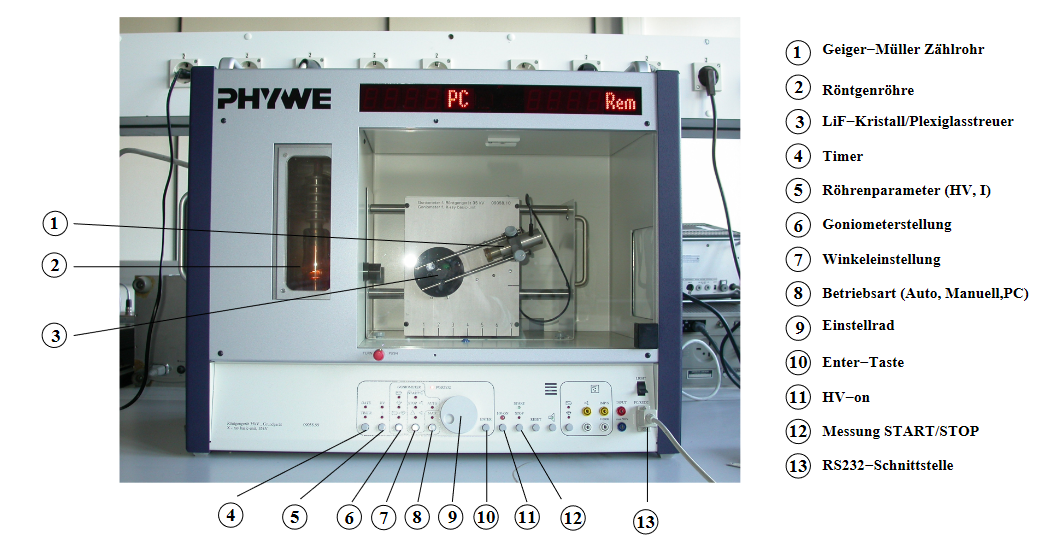
\includegraphics[width=14cm, keepaspectratio]{Compton Effekt Versuchapparatur}
    \caption{Rönthgenröhre}
    \label{fig:Rönthgenröhre}
 \end{figure}
Die hier verwendete Versuchsapparatur besteht aus einer Kupfer-Rönthgenröhre, einem Lif-Kristall bzw. einem Plexiglasstreuer mit verstellbarem Winkel und einem darum drehbar gelagerten Geiger-Müller-Zählrohr. Zusätzlich kann ein Absorber eingesetzt werden um die Transmission zu messen. Die Apparatur kann im Hinblick auf Integrationszeit, Kristallwinkel und Drehmodus wahlweise über einen Computer oder manuell gesteuert werden. \\
Zunächst wird das Emmissionsspektrum der Kupfer Rönthgenröhre durch Veränderung des Kristallwinkels in $\Delta \alpha=0.1$° Abständen bei einer Integrationszeit von $t=300$ s aufgenommen. Anschließend wird bei gleicher Intervalllänge mit einer Integrationszeit von $t=200$ s die Zählrate der Rönthgenstrahlung sowohl mit als auch ohne Aluminium Absorber gemessen um die Transmission in Abhängigkeit von der Wellenlänge zuu untersuchen. Zuletzt werden zur Bestimmung der Compton-Wellenlänge die Intensität unter verschiedenen Bedingungen erhoben. Zum einen die Intensität ohne Aluminium Absorber.Zum anderen die Intensität mit einem Aluminium Absorber zwischen Rönthgenröhre und Plexiglasstreuer und mit dem Absorber zwischen Streukörper und Zählrohr. Alle drei Messungen werden mit einer Integrationszeit von $t=300$ s durchgeführt. 
